\documentclass{article}
\usepackage{graphicx} % Required for inserting images
\usepackage{amsmath,amssymb}
\usepackage{pgfplots}
\graphicspath{./images}
\usepackage{array}
\usepackage{hyperref}
\usepackage{listings}

\title{TP2 EDP}
\author{Sacha}
\date{June 2023}

\begin{document}

\maketitle

\section{Vérification}

\subsection{Le Laplacien}

$\Omega$ est le cercle unité et $\partial(\Omega) = \Gamma_D \cup \Gamma_N \cup \Gamma_F$

$\Gamma_D = \{ x = (cos(\theta),sin(\theta)), \theta \in (0,\frac{\pi}{2}) \}$

$\Gamma_N = \{ x = (cos(\theta),sin(\theta)), \theta \in (\frac{\pi}{2},\pi) \}$

$\Gamma_F = \{ x = (cos(\theta),sin(\theta)), \theta \in (\pi,2 \pi) \}$



$$\begin{cases}
    -\Delta u = f \\
    u = g \text{ sur } \Gamma_D\\
    \frac{\partial u}{\partial n} = m \text{ sur } \Gamma_N\\
    u + \frac{\partial u}{\partial n} = l \text{ sur } \Gamma_F
\end{cases}$$

2. Soit $v \in H^1_0(\Omega)$ une fonction test. Multiplions $v$ des deux côtés de la première égalité et intégrons l'équation

\begin{align*}
    -\int_{\Omega} \Delta u v &= \int_{\Omega} f v \\
    \text{En appliquant la formule de} &\text{ Green, on obtient} \\
    \int_{\Omega}  \nabla u \nabla v - \int_{\partial(\Omega)} \frac{\partial u}{\partial n} v &= \int_{\Omega} f v \\
    \text{Or $v = 0$ sur $\partial(\Omega)$} &\text{ car $v \in H_0^1(\Omega)$} \\
    \text{Donc, } \int_{\Omega} \nabla u \nabla v &= \int_{\Omega} fv
\end{align*}

Après assemblage du maillage sur Gmsh voici le maillage qu'on obtient:
\includegraphics[scale=0.75]{images/meshgrid_circle.png}

En utilisant feelpp\_toolbox\_coefficientformpdes, on obtient la solution suivante:

\includegraphics[scale=0.75]{images/cercle_dirichlet_robin_fourier_1_0_up.png}

La barre en bas à droite correspond à l'échelle des valeurs. Plus la couleur d'un point est bleue, plus sa valeur en u est proche de 0. Et inversement, plus la couleur est jaune, plus sa valeur est proche du maximum de u (0.874).

On remarque que le bord du demi disque supérieur est égale à 0, ça correspond en fait aux conditions de Neumann et Dirichlet.

3. Pour que le $u$ de notre équation soit égal à $sin(\pi x) cos(\pi y)$ on doit avoir:

$f(x,y) = -2 \pi^2 sin(\pi x) cos(\pi y)$

$g = sin(\pi x) cos(\pi y)$

$m = -\pi y * cos(\pi x)cos(\pi y)-\pi x*sin(\pi x) sin(\pi y)$

$l = g+m$

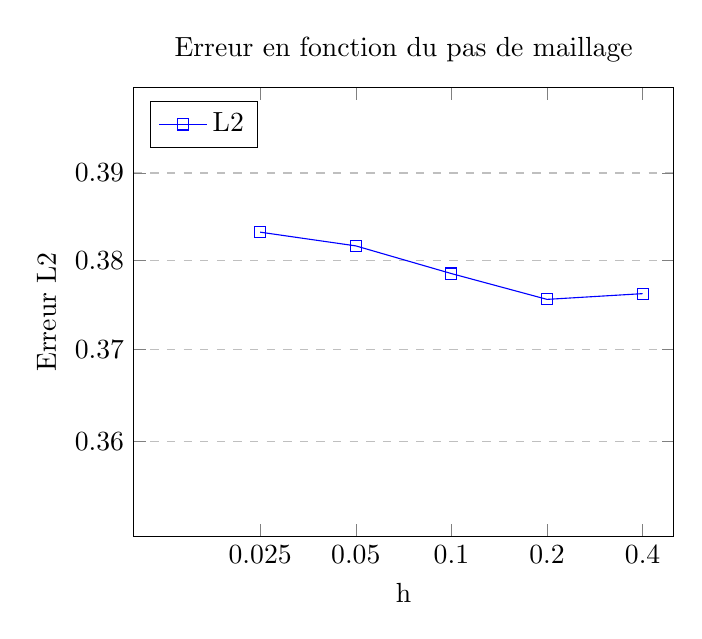
\begin{tikzpicture}
\begin{axis}[
    title={Erreur en fonction du pas de maillage},
    xmode=log,
    log ticks with fixed point,
    ymode=log,
    log ticks with fixed point,
    xlabel={h},
    ylabel={Erreur L2},
    xmin=0.01, xmax=0.5,
    ymin=0.35, ymax=0.4,
    xtick={0.025,0.05,0.1,0.2,0.4},
    ytick={0.36,0.37,0.38,0.39},
    legend pos=north west,
    ymajorgrids=true,
    grid style=dashed,
]

\addplot[
    color=blue,
    mark=square,
    ]
    coordinates {
    (0.4 , 3.7626043526292224e-01)(0.2,3.7560744476157265e-01)(0.1,3.7851697033548642e-01)(0.05,3.8162954415792721e-01)(0.025,3.8324343471680672e-01)
    };
    \legend{L2}
    
\end{axis}
\end{tikzpicture}

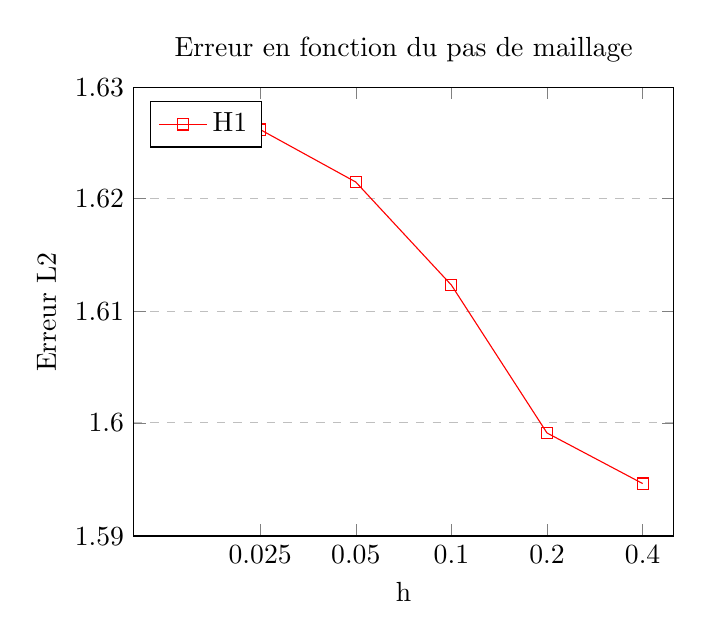
\begin{tikzpicture}
\begin{axis}[
    title={Erreur en fonction du pas de maillage},
    xmode=log,
    log ticks with fixed point,
    ymode=log,
    log ticks with fixed point,
    xlabel={h},
    ylabel={Erreur L2},
    xmin=0.01, xmax=0.5,
    ymin=1.59, ymax=1.63,
    xtick={0.025,0.05,0.1,0.2,0.4},
    ytick={1.59,1.60,1.61,1.62,1.63},
    legend pos=north west,
    ymajorgrids=true,
    grid style=dashed,
]
\addplot[
    color=red,
    mark=square,
    ]
    coordinates {
    (0.4,1.5945754308451690e+00)(0.2,1.5990264017217748e+00)(0.1,1.6122403538907137e+00)(0.05,1.6215411772849726e+00)(0.025,1.6263099266864782e+00)
    };
    \legend{H1}
\end{axis}
\end{tikzpicture}


\subsection{Fonctions peu régulières}

2) Calculons $\frac{\partial u}{\partial r}$ et $\frac{\partial u}{\partial \theta}$

$\frac{\partial u}{\partial r} = \frac{2}{3}r^{-\frac{1}{3}}sin(\frac{2}{3} \theta)$

$\frac{\partial u}{\partial \theta} = -\frac{2}{3}r^{\frac{2}{3}}cos(\frac{2}{3} \theta)$

Or:

$\frac{\partial u}{\partial r}^2 \leq \left(\frac{2}{3}\right)^2 sin^2(\frac{2}{3} \theta)$

$\frac{\partial u}{\partial \theta}^2 = \left( -\frac{2}{3} \right) cos^2(\frac{2}{3} \theta)$

Car $r < 1$

De plus, $\Omega$ est bornée, donc $sin^2$ et $cos^2$ sont intégrables à une constante près.

D'où $u \in H^1(\Omega)$

Maintenant, si on a $\theta$ tel que $(\frac{2}{3} \theta) \neq 0$. Alors on a $r^{-\frac{1}{3}} \to 0$ quand $r \to 0$

Donc $\frac{\partial u}{\partial r} \to 0$ quand $r \to 0$. On en déduit que le gradient n'est pas borné à l'origine, et donc $u \in H^2$ puisque $\frac{\partial u}{\partial r}$ n'est pas dérivable en 0.


3)

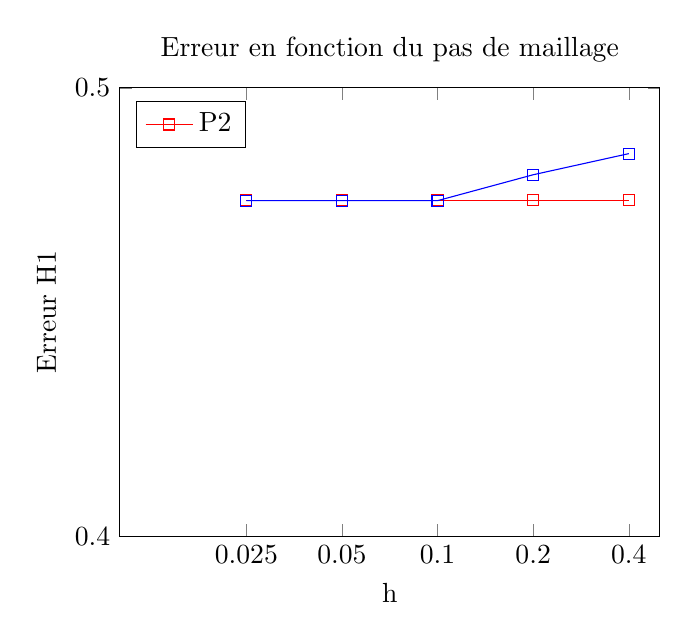
\begin{tikzpicture}
\begin{axis}[
    title={Erreur en fonction du pas de maillage},
    xmode=log,
    log ticks with fixed point,
    ymode=log,
    log ticks with fixed point,
    xlabel={h},
    ylabel={Erreur H1},
    xmin=0.01, xmax=0.5,
    ymin=0.4, ymax=0.5,
    xtick={0.025,0.05,0.1,0.2,0.4},
    ytick={0.4,0.5},
    legend pos=north west,
    ymajorgrids=true,
    grid style=dashed,
]
\addplot[
    color=red,
    mark=square,
    ]
    coordinates {
    (0.4,4.7279117435887219e-01)(0.2,4.7279117435887219e-01)(0.1,4.7279117435887219e-01)(0.05,4.7279117435887219e-01)(0.025,4.7279117435887219e-01)
    };
    \legend{P1}
\addplot[
    color=blue,
    mark=square,
    ]
    coordinates {
    (0.4,4.8390615814071947e-01)(0.2,4.7884006041386845e-01)(0.1,4.7270440620183463e-01)(0.05,4.7270440620183463e-01)(0.025,4.7270440620183463e-01)
    };
    \legend{P2}
\end{axis}
\end{tikzpicture}

On remarque que l'erreur stagne au bout d'un certain pas de maillage

La toolbox utilisée pour cette section est dans le fichier cercle\_trois\_quart.json

\section{Méthode de stabilisation}

En testant plusieurs valeurs de $\epsilon$ on obtient les résultats suivants:

\includegraphics[width=0.8\textwidth]{images/eps10.png}
\begin{center}
    \textbf{Figure 1: $\epsilon$ = 10}
\end{center}
\includegraphics[width=0.9\textwidth]{images/esp1.png}
\begin{center}
    \textbf{Figure 2: $\epsilon$ = 1}
\end{center}
\includegraphics[width=0.8\textwidth]{images/eps1e-1.png}
\begin{center}
    \textbf{Figure 3: $\epsilon$ = 1e-1}
\end{center}
\includegraphics[width=0.9\textwidth]{images/eps1e-3.png}
\begin{center}
    \textbf{Figure 4: $\epsilon$ = 1e-3}
\end{center}

On remarque que plus $\epsilon$ est proche de 0, plus la valeur maximale de la solution (Le point le plus jaune) se rapproche d'un coin du carré.

2) Pour $\epsilon = 10$ ou $1e-1$, on ne remarque pas de changements significatifs entre les différentes méthodes.

\includegraphics[width=0.9\textwidth]{images/eps10.png}
\begin{center}
    \textbf{Figure 5: $\epsilon$ = 10 avec SUPG}
\end{center}
\includegraphics[width=0.8\textwidth]{images/eps10_gals.png}
\begin{center}
    \textbf{Figure 6: $\epsilon$ = 10 avec GaLS}
\end{center}
\includegraphics[width=0.9\textwidth]{images/eps10_no_stabilization.png}
\begin{center}
    \textbf{Figure 7: $\epsilon$ = 10 sans méthode de stabilisation}
\end{center}

Cependant, si on prend $\epsilon = 1e-3$, on obtient un résultat très différent.

\includegraphics[width=0.9\textwidth]{images/eps1e-3.png}
\begin{center}
    \textbf{Figure 8: $\epsilon$ = 1e-3 avec SUPG}
\end{center}
\includegraphics[width=0.8\textwidth]{images/eps1e-3_gals.png}
\begin{center}
    \textbf{Figure 9: $\epsilon$ = 1e-3 avec GaLS}
\end{center}
\includegraphics[width=0.9\textwidth]{images/eps1e-3_no_stabilization.png}
\begin{center}
    \textbf{Figure 10: $\epsilon$ = 1e-3 sans méthode de stabilisation}
\end{center}

3.1) Pour vérifier l'ordre de convergence, nous allons considérer une fonction $u(x,y) = x^2+y^2$

Pour que u soit solution du problème, on doit avoir $f = -4e-3+2*x+2*y+x^2+y^2$ et $g = x^2+y^2$ si on prend $\epsilon = 1e-3$, $\beta = (1,1)^T$, $\mu = 1$ et $g=0$.

Regardons les erreurs en normes $L^2$ et $H^1$:

\begin{tabular}{c|c|c}
    h & $L^2$ & $H^1$ \\
    0.4   &  1.8799026774634953e-01 &  2.2682461643710003e-02 \\
    0.2   &  1.1270157838966860e-01 &  8.2928153375460677e-03 \\
    0.1   &  5.7989554719951569e-02 &  1.9807126752690446e-03 \\
    0.05  &  2.9143380172362593e-02 &  4.9159706734286835e-04 \\
    0.025 &  1.4476276503802189e-02 & 1.2284868096793368e-04
\end{tabular}

\textbf{Table 1: Erreur en norme $L^2$ et $H^1$ pour différent pas de maillage avec une base de fonctions $\mathbb{P}_1$}

\begin{tabular}{c|c|c}
    h & $L^2$ & $H^1$ \\
    0.4   &  7.1088742768433036e-15 &  9.1605437148933129e-16 \\
    0.2   &  1.3057911970147188e-14 &  4.7978347293371833e-16 \\
    0.1   &  2.3735140893920529e-14 &  5.8111735674615155e-16 \\
    0.05  &  3.9026536236342233e-14 &  1.4540753830744363e-15 \\
    0.025 &  7.4083789924857955e-14 &  2.7957426964335838e-15
\end{tabular}

\textbf{Table 2: Erreur en norme $L^2$ et $H^1$ pour différent pas de maillage avec une base de fonctions $\mathbb{P}_2$}

En utilisant la section Statistics de la toolbox feel++, nous pouvons également calculer la norme $H^1$ de notre solution. Feel++ nous donne ce résultat:

$$||u||_{H^1} \approx 1.81$$

On a donc bien:

$$||u-u_h||_{L^2} \leq h^{\frac{1}{2}}||u||_{H^1}$$

Avec $h$, le pas du maillage. Ce qui confirme la convergence d'ordre $\frac{1}{2}$ .

La toolbox associée à cette partie est trouvable dans le fichier adr\_manufacturee.cfg et adr\_manufacturee.json du dossier adr.

3.2) Voici la solution du problème après avoir appliqué une méthode de stabilisation GaLS.

\includegraphics[]{images/L_results_P2.png}
\begin{center}
    \textbf{Figure 11: Solution approximé de u sur un maillage en forme de L}
\end{center}

Sur le bord gauche, nous remarquons que la solution est tout le temps égale à 1, comme la condition de Dirichlet que l'on a imposé.

On remarque aussi que sur les autre bords, la solution est nulle (excepté le bord bas), ça correspond à la condition de Dirichlet homogène. Et le bord bas corredpond à la condition de Neumann homogène.

La toolbox utilisée pour générer cette solution est trouvable dans le fichier adr\_L.cfg et adr\_L.json dans le dossier adr. Le maillage utilisé s'appelle L.geo

\section{Stokes}

1) Pour que la solution de Kovsznay soit solution du problème, on doit calculer f tel que:

$$- \Delta u + \nabla p = f$$

et 

$$u=g \text{ sur } \partial \Omega$$

Intéressons-nous à la première équation:

$$\Delta u = \Delta u_1 e_1+ \Delta u_2 e_2$$

avec $u_i$ la i-ème coordonnée du vecteur u, et $e_i$ le i-ème vecteur de la base canonique.

\begin{align*}
    \frac{\partial u_1}{\partial x} &= -\lambda e^{\lambda x} cos(2 \pi y)& \; \frac{\partial u_1}{\partial y} &= 2 \pi e^{\lambda x} sin(2 \pi y) \\
    \frac{\partial^2 u_1}{\partial x^2} &= - \lambda^2 e^{\lambda x} cos(2 \pi y)& \; \frac{\partial^2 u_1}{\partial y^2} &= 4 \pi^2 e^{\lambda x} cos(2 \pi y)
\end{align*}

On a donc $\Delta u_1 = (4 \pi^2-\lambda^2) e^{\lambda x} cos(2 \pi y)$

\begin{align*}
    \frac{\partial u_2}{\partial x} &= \frac{\lambda^2}{2 \pi} e^{\lambda x} sin(2 \pi y)& \; \frac{\partial u_2}{\partial y} &= \lambda e^{\lambda x} cos(2 \pi y) \\
    \frac{\partial^2 u_2}{\partial x^2} &= - \lambda^3 e^{\lambda x} sin(2 \pi y)& \; \frac{\partial^2 u_2}{\partial y^2} &= - 2 \lambda \pi e^{\lambda x} sin(2 \pi y)
\end{align*}

Finalement, on a:

$$\Delta u = \begin{pmatrix}
(4 \pi^2-\lambda^2) e^{\lambda x} cos(2 \pi y) \\
(\frac{\lambda^3}{2 \pi}-2 \lambda \pi) e^{\lambda x} sin(2 \pi y)
\end{pmatrix}$$

Calculons $\nabla p$

$p = -\frac{e^{2 \lambda x}}{2} + C$

$\frac{\partial p}{\partial x} = -\lambda e^{2 \lambda x}$

Comme il n'y a pas de y dans $p$, il vient immédiatement que $\frac{\partial p}{\partial y} = 0$.

Et donc:

$\nabla p = \begin{pmatrix}
    -\lambda e^{2 \lambda x} \\
    0
\end{pmatrix}$

Finalement on a:

\begin{align*}
    f &= \begin{pmatrix}
(4 \pi^2-\lambda^2) e^{\lambda x} cos(2 \pi y) \\
(\frac{\lambda^3}{2 \pi}-2 \lambda \pi) e^{\lambda x} sin(2 \pi y)
\end{pmatrix} + \begin{pmatrix}
    -\lambda e^{2 \lambda x} \\
    0
\end{pmatrix} \\
 &= \begin{pmatrix}
(4 \pi^2-\lambda^2) e^{\lambda x} cos(2 \pi y) -\lambda e^{2 \lambda x} \\
(\frac{\lambda^3}{2 \pi}-2 \lambda \pi) e^{\lambda x} sin(2 \pi y)
\end{pmatrix}
\end{align*}

Maintenant, déterminons $C$ tel que $p$ soit de moyenne nulle, c'est à dire:

$$\int_{\Omega} p = 0$$

Comme $\Omega$ est un rectangle, on a l'égalité suivante:

\begin{align*}
    \int_{\Omega} p &= \int^1_{-0.5} \int^{1.5}_{-0.5} \frac{-e^{2 \lambda x}}{2} + C dy dx \\
    &= \int^1_{-0.5} \left(\frac{-e^{2 \lambda x}}{2} + C\right) \int^{1.5}_{-0.5} dy dx \\
    &= \int^1_{-0.5} \left(\frac{-e^{2 \lambda x}}{2} + C\right) \left[ y \right]^{1.5}_{-0.5} dx \\
    &= 2 \int^1_{-0.5} \left(\frac{-e^{2 \lambda x}}{2} + C\right) dx \\
    &= 2 \left[ \frac{- e^{2 \lambda x}}{4 \lambda} + Cx \right]^1_{-0.5} \\
    &= 2 \left( \frac{- e^{2 \lambda}}{4 \lambda} + C + \frac{e^{-\lambda}}{4 \lambda} + \frac{C}{2}\right) \\
    &= \frac{-e^{2 \lambda} + e^{-\lambda}} {2 \lambda} + 3C
\end{align*}

Or on a:

\begin{align*}
    \frac{-e^{2 \lambda} + e^{-\lambda}} {2 \lambda} + 3C &= 0 \\
    3C &= \frac{ e^{2 \lambda} - e^{-\lambda}} {2 \lambda} \\
    C &= \frac{ e^{2 \lambda} - e^{-\lambda}} {6 \lambda}
\end{align*}

2) Voici la formulation variationnelle pour le problème de Stokes:

On cherche $(u,p)$ dans $H^1_0 \times L^2_*$ avec $L^2_*$ l'ensemble des fonctions de carré intégrable telle que $\int_{\Omega} p = 0$.

$$\int_{\Omega} \nabla u:\nabla v - \int_{\Omega} p \nabla \cdot v = \int_{\Omega} f \cdot v $$

$$\int_{\Omega}q \nabla \cdot u = 0 $$

$\forall v \in H^1_0(\Omega)$ et $\forall q \in L^2_*$

3) En choisissant, une base $\mathbb{P}_1/\mathbb{P}_1$ voici les solutions obtenues:

\includegraphics[scale=0.75]{images/mass_pressure_P1_P1.png}
\begin{center}
    \textbf{Figure 12: Solution approchée de p avec une erreur $L^2$ de: 1.5577586580821336e+06}
\end{center}
\includegraphics[scale=0.75]{images/momentum_velocity_P1_P1.png}
\begin{center}
    \textbf{Figure 13: Solution approchée de u avec une erreur $L^2$ de: 7.4786283012603649e-01}
\end{center}

On remarque que la méthode a du mal à converger vers la solution exacte de p

4) Maintenant en utilisant la méthode $\mathbb{P}_2/\mathbb{P}_1$, on obtient les résultats suivants:

\includegraphics[scale=0.75]{images/momentum_velocity_P2_P1.png}
\begin{center}
    \textbf{Figure 14: Solution approchée de u avec une base $\mathbb{P}_2/\mathbb{P}_1$}
\end{center}

\includegraphics[scale=0.75]{images/mass_pressure_P2_P1.png}
\begin{center}
    \textbf{Figure 15: Solution approchée de p avec une base $\mathbb{P}_2/\mathbb{P}_1$}
\end{center}

\end{document}
